% prime.tex — حواف العدّ والحساب — Prime — النسخة النهائية للرفع
% Compiler: XeLaTeX
% Figures — all lowercase p:
% prime1.png = Identity Card
% primeB1.png = B: D1 | primeB2.png = B: Density | primeB3.png = B: Gap frequencies
% primeC1.png = C: D1 | primeC2.png = C: Density | primeC3.png = C: Gap frequencies
% primeD1.png = D: D1 | primeD2.png = D: Density | primeD3.png = D: Gap frequencies

\documentclass[12pt,a4paper]{article}
\usepackage{amsmath,amssymb}
\usepackage{graphicx}
\usepackage{booktabs}
\usepackage{array}
\usepackage[margin=2.2cm]{geometry}
\usepackage{xcolor}
\usepackage{float}
\usepackage{fontspec}
\usepackage{polyglossia}

\setmainlanguage[numerals=maghrib]{arabic}
\setotherlanguage{english}
\setmainfont{Amiri}

% --- الهيدر والفوتر ---
\usepackage{fancyhdr}
\pagestyle{fancy}
\fancyhf{}
\fancyhead[L]{\small \textenglish{Edges of Counting and Computation — Prime}}
\fancyhead[R]{\small \textenglish{M. N. Al-Jabri (2026)}}
\fancyfoot[L]{\scriptsize \textenglish{Abdulla M. N. Al-Jabri | ORCID: 0009-0003-3319-3822}}
\fancyfoot[C]{\scriptsize \textenglish{Zenodo DOI: to be assigned}}
\fancyfoot[R]{\small \thepage}
\renewcommand{\headrulewidth}{0.4pt}
\renewcommand{\footrulewidth}{0.4pt}

\fancypagestyle{firstpage}{
  \fancyhf{}
  \fancyfoot[C]{عبدالله محمد ناصر الجبري — حواف العدّ والحساب — Prime — \thepage}
  \renewcommand{\headrulewidth}{0pt}
  \renewcommand{\footrulewidth}{0pt}
}

\AtBeginDocument{\providecommand{\UseMathForPositioningText}{}}
\title{\textbf{حواف العدّ والحساب — \textenglish{Prime}}}
\author{عبدالله محمد ناصر الجبري \\
صنعاء، اليمن \\
\textenglish{ORCID: 0009-0003-3319-3822} \\
\textenglish{Email: jabri62018@gmail.com} \\
\textenglish{Portal: \url{https://jabri-com.vercel.app}} \\
\textenglish{Zenodo DOI: to be assigned on deposit}}
\date{21 نوفمبر 2026م}

\begin{document}
\maketitle
\thispagestyle{firstpage}

\begin{center}
\textbf{نعدّ الأوليات، نحسب حوافها، ونختبر ما إذا كانت تحمل بنية أو ذاكرة.}
\end{center}

\begin{center}
\small عبدالله محمد ناصر الجبري \quad $\cdot$ \quad صنعاء، اليمن \quad $\cdot$ \quad \textenglish{ORCID: 0009-0003-3319-3822} \quad $\cdot$ \quad \textenglish{Email: jabri62018@gmail.com}
\end{center}

\vspace{0.5cm}

% ==========================================
\section{الملخص (\textenglish{Abstract})}
تستقصي هذه الورقة السلوك الإحصائي والبنيوي للفجوات (الحواف) بين الأعداد الأولية المتتالية $g_n = p_{n+1} - p_n$ وصولاً إلى الحد الحسابي $N = 10^9$ (مليار). نقوم بتتبع دالة الانحراف $D_1(x) = \pi(x) - \mathrm{Li}(x)$، وكثافة الأوليات $\rho_k$، وتوزيع تكرارات الفجوات عبر ثلاثة نطاقات تجريبية مستقلة ($B, C, D$). تُظهر النتائج الحسابية بقاء $D_1(x)$ سالبًا عبر كامل النطاق المفحوص، وتناقصًا مستمرًا في الكثافة متوافقًا مع مبرهنة الأعداد الأولية، بالإضافة إلى حدوث تحول ملحوظ في ترتيب تكرار الحواف داخل النطاق الأعلى ($D$). نخلص إلى دحض فرضية ثبات ترتيب التكرار، ونصوغ رصدًا تجريبيًا يربط ديناميكية الحواف بتناقص الكثافة دون ادعاء وجود قانون دوري حتمي أو صيغة تنبؤية مغلقة.

% ==========================================
\section{المقدمة والمشكلة والفرضية}
تُعدّ الأعداد الأولية اللبنات الأساسية لنظرية الأعداد، وعلى الرغم من حتمية تعريفها، فإن توزيعها الموضعي يظهر سلوكًا شبه عشوائي يثير تساؤلات جوهرية حول وجود ارتباطات خفية بين الفجوات المتتالية.

\begin{itemize}
    \item \textbf{المشكلة البحثية:} هل تمتلك الفجوات بين الأعداد الأولية المتتالية «ذاكرة» إحصائية أو بنية انتقال متكررة؟
    \item \textbf{الفرضية الصفرية (قبل الحساب):} افترضنا مبدئيًا أن أحجام الحواف تتصرف كمتغيرات مستقلة إحصائيًا، وأن الترتيب النسبي لتكرار الحواف الأكثر شيوعًا (مثل $2, 4, 6$) يظل مستقرًا عبر النطاقات العددية المتصاعدة.
    \item \textbf{منهجية الاختبار:} فحص ما إذا كانت فئة حجم الحافة الحالية $g_n$ تحمل معلومة إحصائية تؤثر في الحافة اللاحقة $g_{n+1}$، ومقارنة استقرار ترتيب التكرار عبر ثلاث تشغيلات حسابية مستقلة ($B$ و $C$ و $D$).
\end{itemize}

\noindent \textbf{تنبيه منهجي:} هذه الورقة تقدم رصدًا تجريبيًا وفرضية مختبرة، وليست مبرهنة ولا حدسية. لا يوجد أي ادعاء يتجاوز $10^9$.

% ==========================================
\section{الهوية الرسمية للبحث}
\begin{figure}[H]
\centering
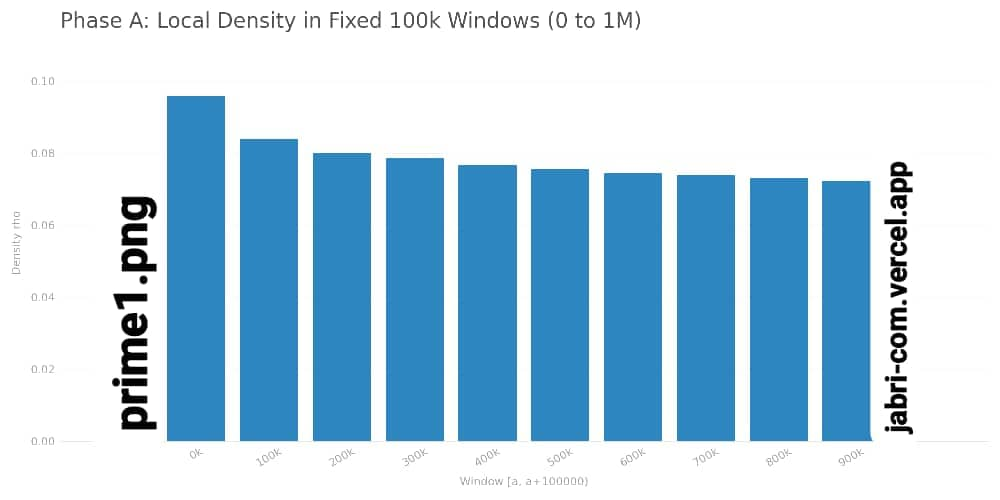
\includegraphics[width=0.92\textwidth]{prime1.png}
\caption{بطاقة الهوية الرسمية لمشروع البحث — \textenglish{Prime}}
\end{figure}

\begin{table}[H]
\centering
\begin{tabular}{ll}
\toprule
\textbf{العنصر} & \textbf{المعتمد} \\
\midrule
الاسم & عبدالله محمد ناصر الجبري \\
الاسم بالإنجليزية & \textenglish{Abdulla M. N. Al-Jabri} \\
العنوان & صنعاء، اليمن \\
\textenglish{ORCID} & \textenglish{0009-0003-3319-3822} \\
البريد الإلكتروني & \textenglish{jabri62018@gmail.com} \\
\textenglish{Zenodo DOI} & \textenglish{to be assigned on deposit} \\
اسم العمل & حواف العدّ والحساب \\
الرمز المرجعي & \textenglish{Prime} \\
التعريف الرياضي & $g_n = p_{n+1} - p_n$ \\
المنهج & استخراج الأوليات، حساب الحواف، والتحليل الإحصائي للنوافذ \\
السؤال البحثي & هل للفجوات ذاكرة؟ \\
التاريخ & 21 نوفمبر 2026م \\
\bottomrule
\end{tabular}
\caption{البيانات الوصفية والمرجعية للورقة البحثية}
\end{table}

% ==========================================
\section{التعريف والاشتقاق الرياضي}

\subsection{تعريف الحافة (\textenglish{Prime Gap})}
تُعرَّف الحافة رقم $n$ بأنها المسافة الحسابية (الفرق) بين عددين أوليين متتاليين:
\[
g_n = p_{n+1} - p_n, \quad \forall n \geq 1
\]

\subsection{خوارزمية استخراج الحواف}
تعتمد العملية الحسابية على ثلاث خطوات صارمة:
\begin{enumerate}
    \item \textbf{الغربال:} تطبيق غربال إراتوستينس (\textenglish{Sieve of Eratosthenes}) لاستخراج كافة الأعداد الأولية حتى الحد $N = 10^9$، مع استبعاد العدد $1$ صراحةً من مجموعة الأوليات.
    \item \textbf{حساب الفروق:} طرح كل عدد أولي $p_n$ من العدد الأولي الذي يليه مباشرة $p_{n+1}$.
    \item \textbf{الحافة الابتدائية:} الحافة الأولى هي $g_1 = 3 - 2 = 1$، وهي الحالة الفردية الوحيدة في سلسلة الحواف اللانهائية؛ إذ إن كل عدد أولي $p_n > 2$ هو عدد فردي بالضرورة، والفرق بين أي عددين فرديين هو عدد زوجي حتمًا ($g_n \equiv 0 \pmod 2$ لكل $n \geq 2$).
\end{enumerate}

\subsection{مثال مصغر للتوضيح}
\begin{table}[H]
\centering
\begin{tabular}{cccc}
\toprule
\textbf{الرتبة ($n$)} & \textbf{الأولي الحالي ($p_n$)} & \textbf{الأولي التالي ($p_{n+1}$)} & \textbf{الحافة ($g_n$)} \\
\midrule
1 & 2 & 3 & 1 \\
2 & 3 & 5 & 2 \\
3 & 5 & 7 & 2 \\
4 & 7 & 11 & 4 \\
5 & 11 & 13 & 2 \\
\bottomrule
\end{tabular}
\caption{نموذج تطبيقي لحساب الحواف الخمس الأولى}
\end{table}

\subsection{دوال العدّ والانحراف والكثافة}
لقياس التباين بين التوزيع الفعلي للأوليات والتقديرات التحليلية، نعتمد الدوال التالية:
\begin{itemize}
    \item $\pi(x)$: دالة عدّ الأوليات الفعلية التي تقل عن أو تساوي $x$.
    \item $\mathrm{Li}(x) = \mathrm{Ei}(\ln x) - \mathrm{Ei}(\ln 2) = \int_2^x \frac{dt}{\ln t}$: التكامل اللوغاريتمي.
    \item $x / \ln x$: التقريب الكلاسيكي لمبرهنة الأعداد الأولية.
    \item $D_1(x) = \pi(x) - \mathrm{Li}(x)$: الانحراف الأول (الفعلي مقابل التكامل اللوغاريتمي).
    \item $D_2(x) = \pi(x) - x/\ln x$: الانحراف الثاني (الفعلي مقابل التقريب الكلاسيكي).
    \item $R(x) = |D_1(x)| / \pi(x)$: الخطأ النسبي للانحراف الأول.
    \item $\rho_k = (\pi(b_k) - \pi(a_k)) / 10^8$: كثافة الأوليات داخل النافذة القياسية $k$ ذات العرض $10^8$.
    \item $\bar{g}_k = 1 / \rho_k$: التباعد المتوسط المقدّر (\textenglish{Estimated Mean Spacing}) داخل النافذة $k$، مشتق من الكثافة، وليس المتوسط المحسوب مباشرة من الفجوات، وهو $\bar{g}_k^{\,\mathrm{actual}} = (1/m_k)\sum_{j=1}^{m_k} g_j$.
    \item $\Delta D_1$: مقدار التغيّر في قيمة $D_1$ مقارنة بنقطة القياس السابقة.
\end{itemize}

\subsection{قاعدة العدّ في النطاق \textenglish{D} وتصنيف فئات \textenglish{M1}}
\textbf{شرط الانتماء للنطاق \textenglish{D}:} تُقبل الحافة $g_n = p_{n+1} - p_n$ ضمن إحصاءات النطاق $D$ فقط إذا تحقق شرط الحد الأعلى: $p_{n+1} > 10^8$ ($100\text{M}$).

\noindent \textbf{فئات التصنيف الحجمي (\textenglish{M1}):}
\begin{itemize}
    \item \textbf{صغيرة (\textenglish{Small}):} $g \leq 6$ (وتشمل القيم $1, 2, 4, 6$).
    \item \textbf{متوسطة (\textenglish{Medium}):} $8 \leq g \leq 14$ (وتشمل القيم $8, 10, 12, 14$).
    \item \textbf{كبيرة (\textenglish{Large}):} $g \geq 16$ (وتشمل كافة القيم الزوجية من $16$ فصاعدًا).
\end{itemize}

\noindent \textbf{الدقة الرياضية للتصنيف:} إن تحديد الفئة المتوسطة بالمدى $[8, 14]$ هو تحديد دقيق وشامل يمنع وجود أي فجوات غير مصنفة بين الفئات؛ نظرًا لأن الحافة الفردية الوحيدة ($g_1 = 1$) محتواة بالكامل داخل الفئة الصغيرة ($g \leq 6$)، وجميع الحواف اللاحقة أعداد زوجية بالضرورة، مما ينفي رياضيًا وجود أي حافة قيمتها $7$ أو $15$ على حدود الفئات.

% ==========================================
\section{التصميم التجريبي والنتائج الحسابية}
تم تقسيم التجربة الحسابية إلى ثلاث مراحل ($B, C, D$) لرصد تطور المؤشرات الثلاثة الأساسية: الانحراف $D_1$، الكثافة $\rho_k$، وتوزيع تكرار الحواف.

\subsection{نتائج التشغيل \textenglish{B}}
توضح الأشكال التالية سلوك الدوال في النطاق الابتدائي/المتوسط $B$:

\begin{figure}[H]
\centering
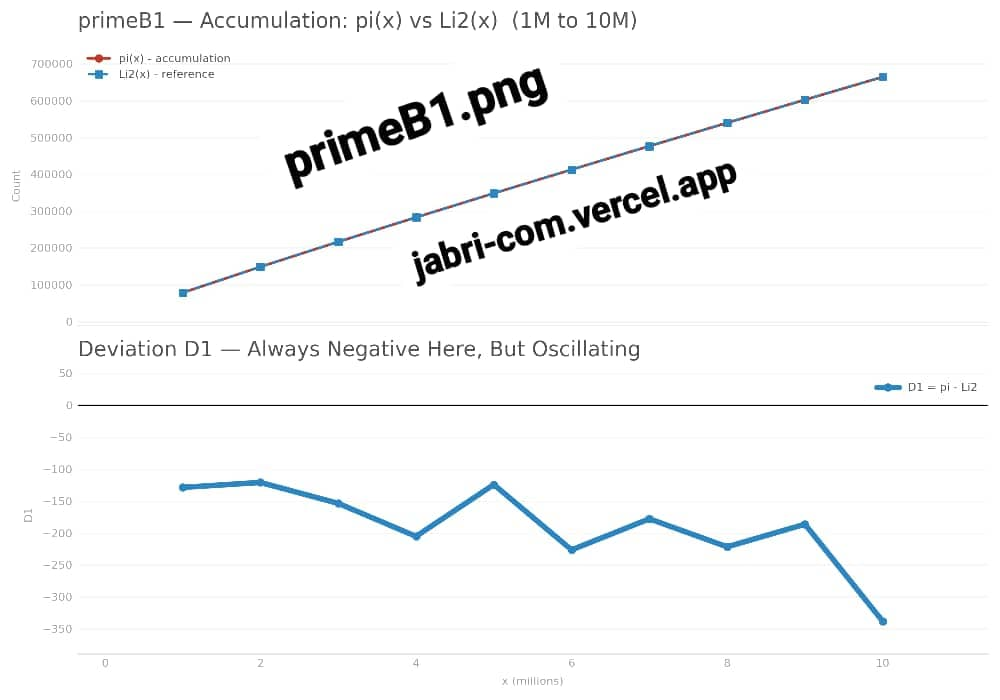
\includegraphics[width=0.85\textwidth]{primeB1.png}
\caption{التشغيل \textenglish{B}: تطور دالة الانحراف $D_1(x)$}
\end{figure}

\begin{figure}[H]
\centering
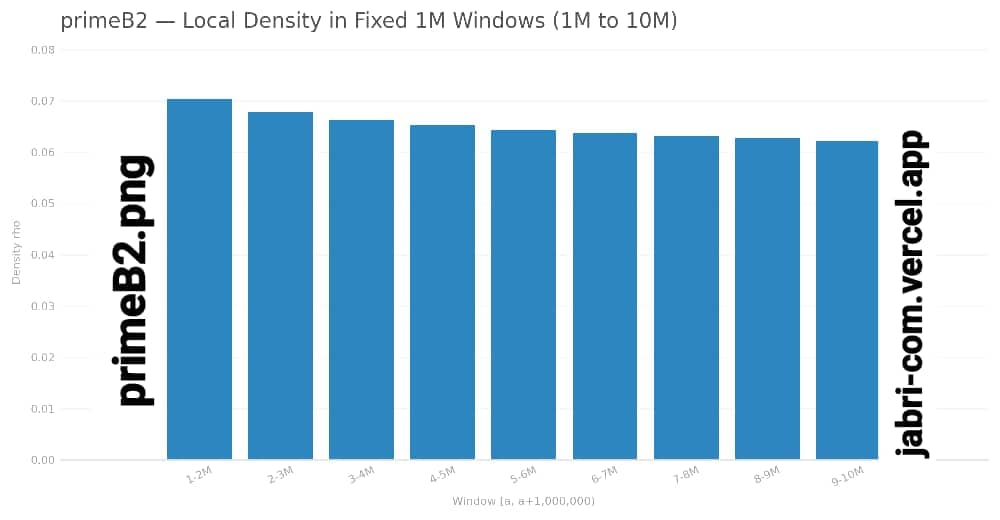
\includegraphics[width=0.85\textwidth]{primeB2.png}
\caption{التشغيل \textenglish{B}: منحنى كثافة الأوليات $\rho_k$}
\end{figure}

\begin{figure}[H]
\centering
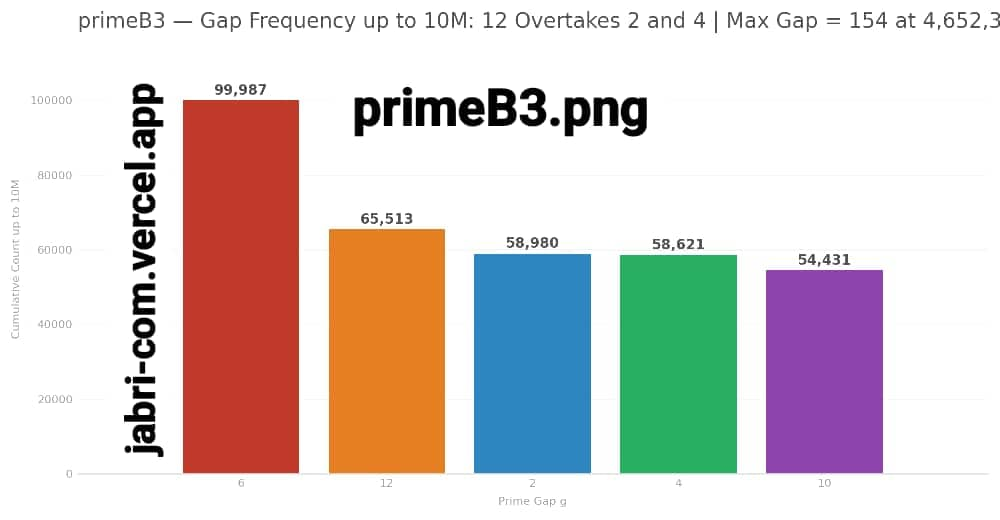
\includegraphics[width=0.85\textwidth]{primeB3.png}
\caption{التشغيل \textenglish{B}: توزيع تكرارات الحواف}
\end{figure}

\subsection{نتائج التشغيل \textenglish{C}}
تُظهر الأشكال أدناه استمرارية الانحراف وتناقص الكثافة في النطاق $C$:

\begin{figure}[H]
\centering
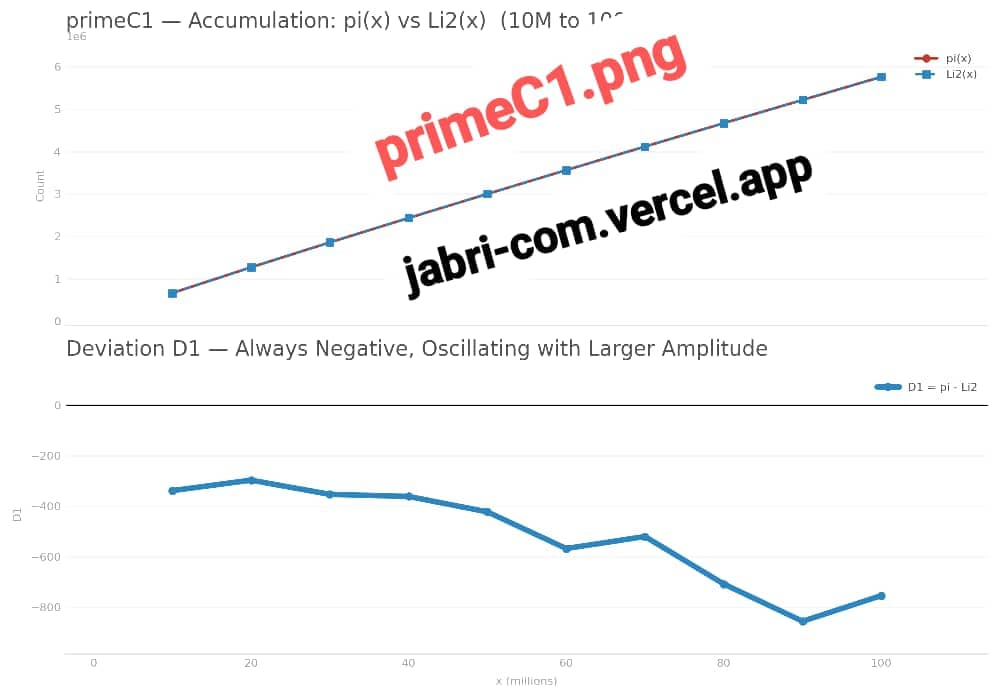
\includegraphics[width=0.85\textwidth]{primeC1.png}
\caption{التشغيل \textenglish{C}: تطور دالة الانحراف $D_1(x)$}
\end{figure}

\begin{figure}[H]
\centering
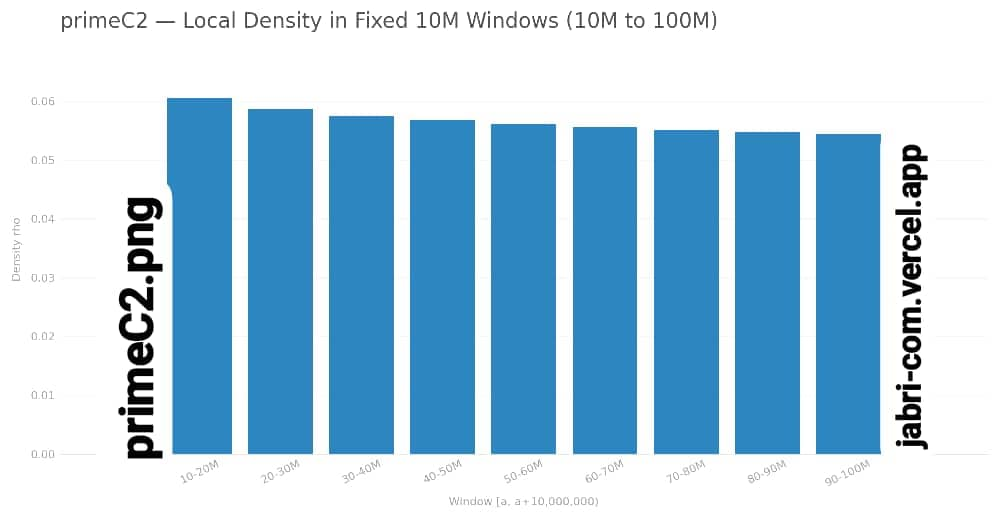
\includegraphics[width=0.85\textwidth]{primeC2.png}
\caption{التشغيل \textenglish{C}: منحنى كثافة الأوليات $\rho_k$}
\end{figure}

\begin{figure}[H]
\centering
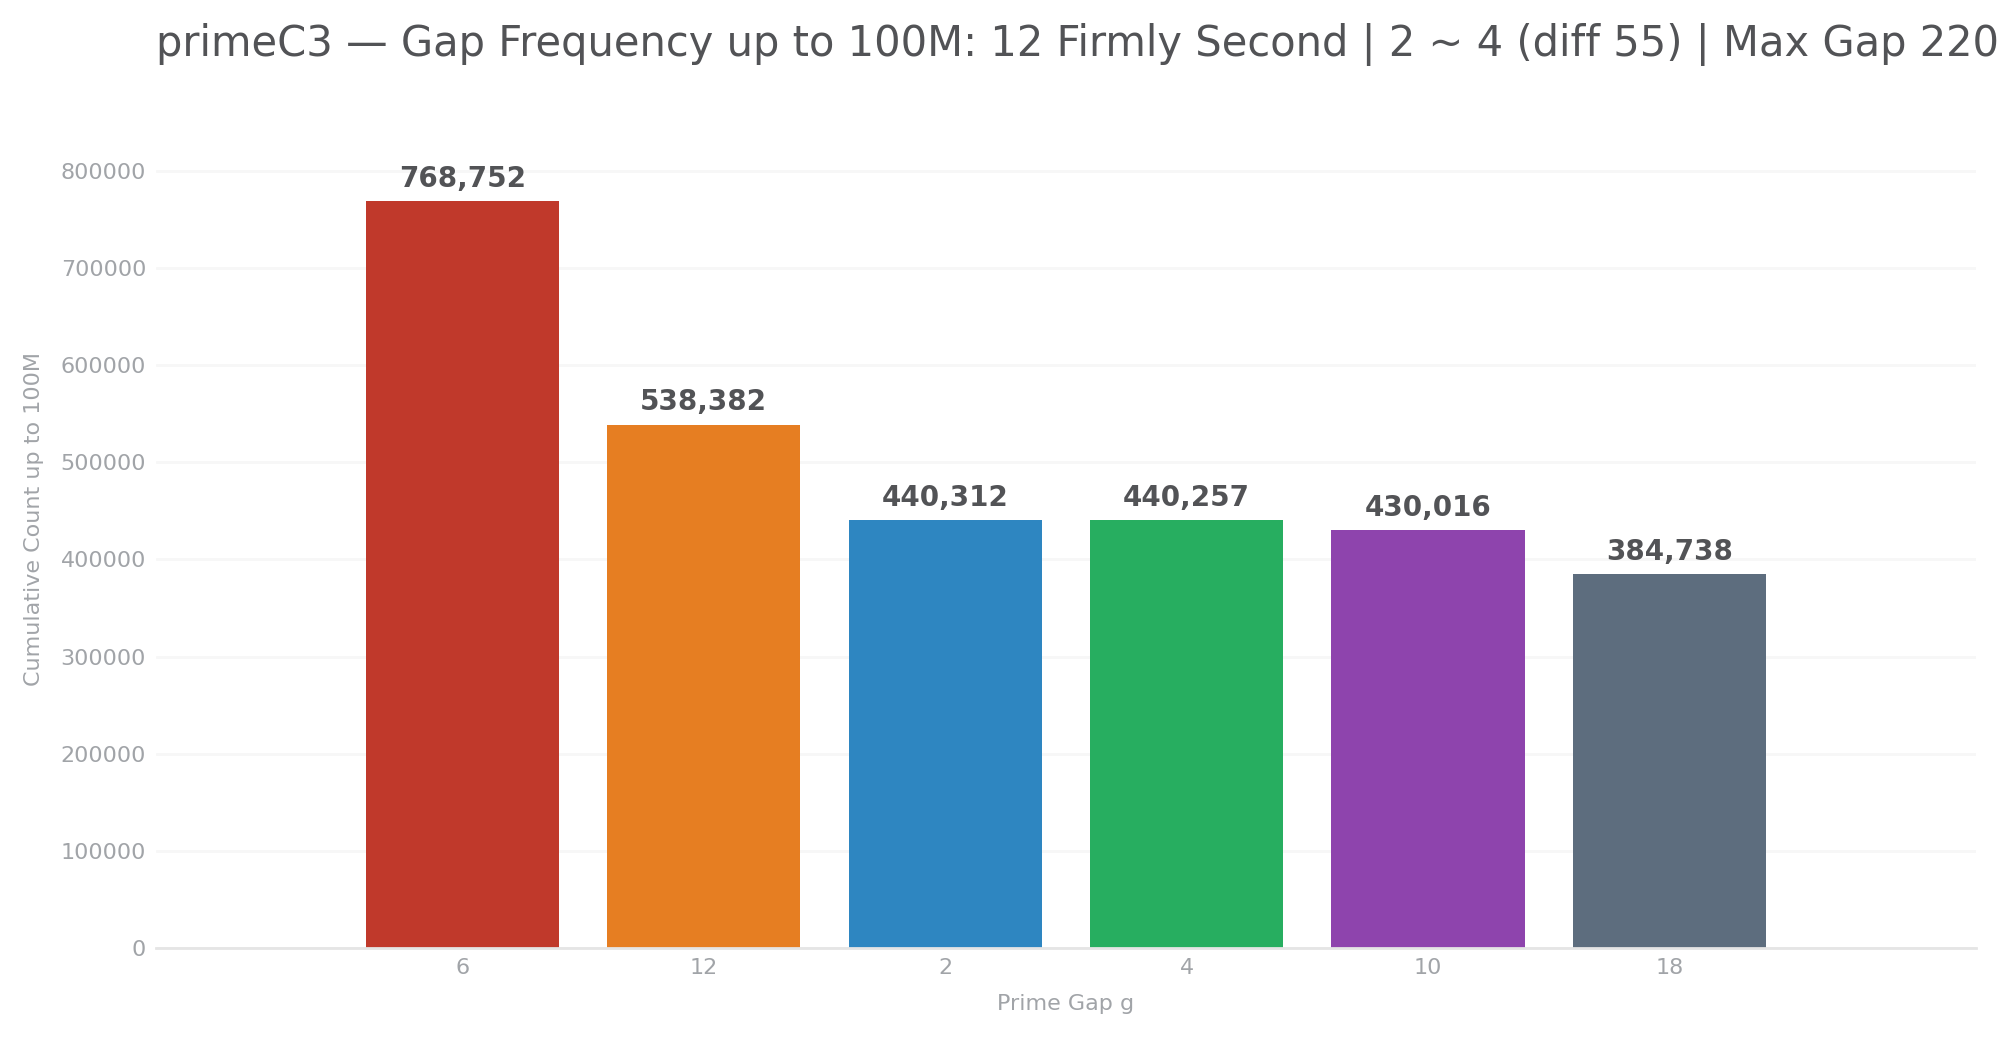
\includegraphics[width=0.85\textwidth]{primeC3.png}
\caption{التشغيل \textenglish{C}: توزيع تكرارات الحواف}
\end{figure}

\subsection{نتائج التشغيل \textenglish{D} (ما فوق $100\text{M}$ حتى $10^9$)}
يمثل النطاق $D$ الاختبار الحاسم للفرضية عند الأعداد الكبيرة:

\begin{figure}[H]
\centering
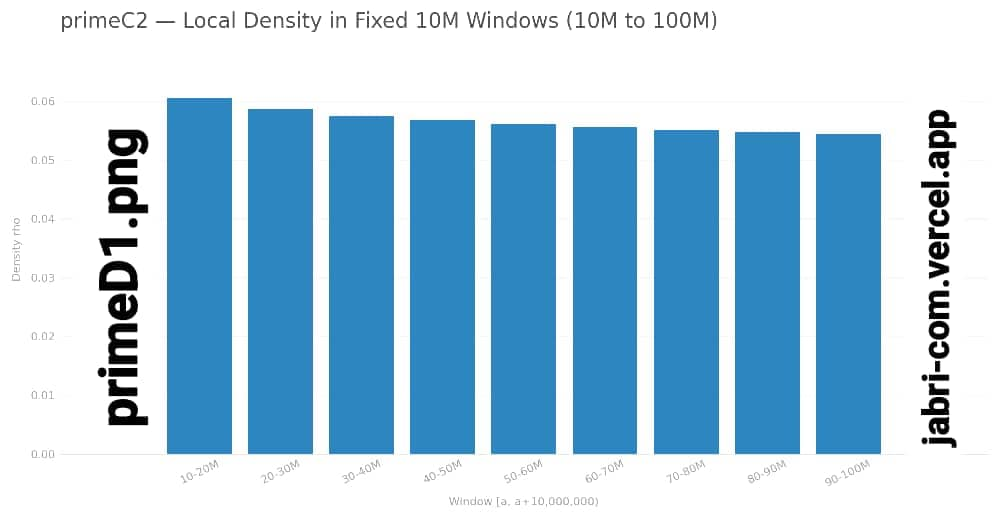
\includegraphics[width=0.85\textwidth]{primeD1.png}
\caption{التشغيل \textenglish{D}: سلوك دالة الانحراف $D_1(x)$ فوق $10^8$}
\end{figure}

\begin{figure}[H]
\centering
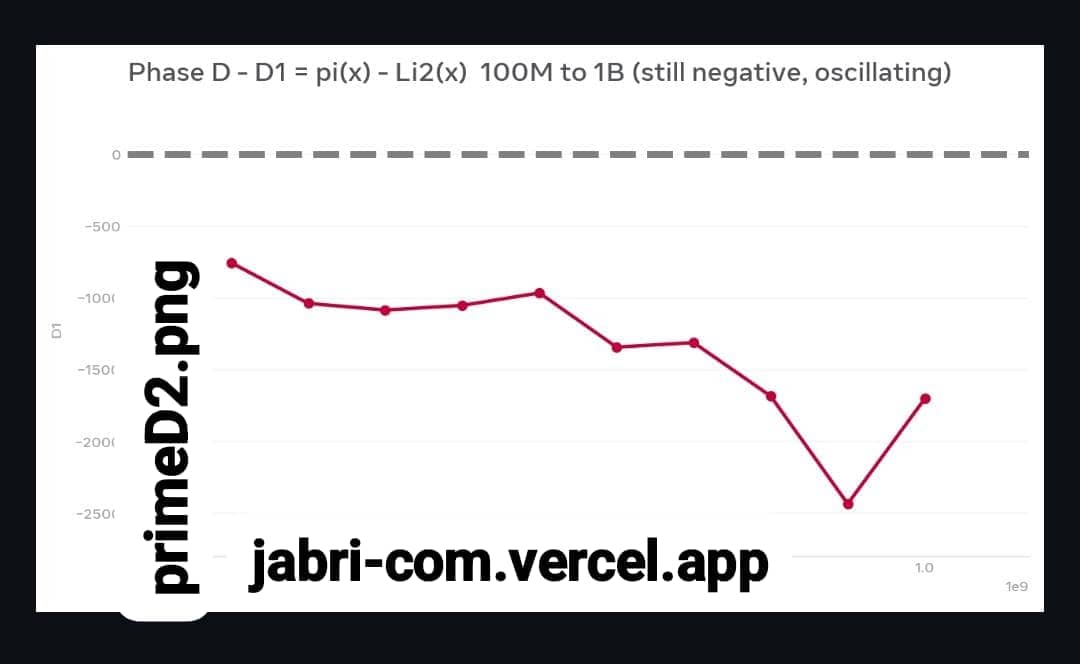
\includegraphics[width=0.85\textwidth]{primeD2.png}
\caption{التشغيل \textenglish{D}: تراجع الكثافة $\rho_k$ وارتفاع متوسط الحافة $\bar{g}_k$}
\end{figure}

\begin{figure}[H]
\centering
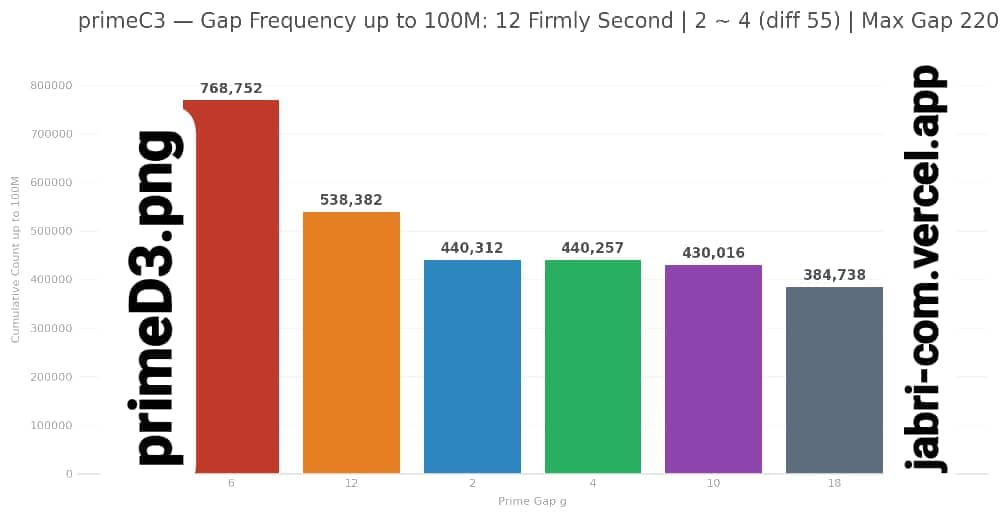
\includegraphics[width=0.85\textwidth]{primeD3.png}
\caption{التشغيل \textenglish{D}: التحول في ترتيب تكرار الحواف}
\end{figure}

% --- الجداول الموثقة ---
\begin{table}[H]
\centering
\small
\begin{tabular}{rrrrrrr}
\toprule
$x$ & $\pi(x)$ & $\mathrm{Li}(x)$ & $D_1$ & $\Delta D_1$ & $D_2$ & $R(x)$ \\
\midrule
$100{,}000{,}000$ & $5{,}761{,}455$ & $5{,}762{,}208.3$ & $-753.3$ & $-753.3$ & $332{,}774.0$ & $0.000131$ \\
$200{,}000{,}000$ & $11{,}078{,}937$ & $11{,}079{,}973.8$ & $-1{,}036.8$ & $-283.5$ & $615{,}308.2$ & $0.000094$ \\
$300{,}000{,}000$ & $16{,}252{,}325$ & $16{,}253{,}408.1$ & $-1{,}083.1$ & $-46.3$ & $882{,}915.9$ & $0.000067$ \\
$400{,}000{,}000$ & $21{,}336{,}326$ & $21{,}337{,}377.0$ & $-1{,}051.0$ & $+32.1$ & $1{,}141{,}420.0$ & $0.000049$ \\
$500{,}000{,}000$ & $26{,}355{,}867$ & $26{,}356{,}831.1$ & $-964.1$ & $+86.9$ & $1{,}393{,}458.7$ & $0.000037$ \\
$600{,}000{,}000$ & $31{,}324{,}703$ & $31{,}326{,}044.207$ & $-1{,}341.207$ & $-377.103$ & $1{,}640{,}014.082$ & $0.000042816$ \\
$700{,}000{,}000$ & $36{,}252{,}931$ & $36{,}254{,}240.999$ & $-1{,}309.999$ & $+31.208$ & $1{,}882{,}917.694$ & $0.000036135$ \\
$800{,}000{,}000$ & $41{,}146{,}179$ & $41{,}147{,}861.2$ & $-1{,}682.2$ & $-372.2$ & $2{,}122{,}021.5$ & $0.000041$ \\
$900{,}000{,}000$ & $46{,}009{,}215$ & $46{,}011{,}647.6$ & $-2{,}432.6$ & $-750.4$ & $2{,}357{,}836.0$ & $0.000053$ \\
$1{,}000{,}000{,}000$ & $50{,}847{,}534$ & $50{,}849{,}233.912$ & $-1{,}699.912$ & $+732.688$ & $2{,}592{,}591.566$ & $0.000033432$ \\
\bottomrule
\end{tabular}
\caption{الجدول التراكمي — كل 100 مليون}
\end{table}

\begin{table}[H]
\centering
\begin{tabular}{rrrr}
\toprule
النافذة & أوليات النافذة & $\rho_k$ & $\bar{g}_k$ \\
\midrule
100M -- 200M & $5{,}317{,}482$ & $0.053175$ & $18.806$ \\
200M -- 300M & $5{,}173{,}388$ & $0.051734$ & $19.330$ \\
300M -- 400M & $5{,}084{,}001$ & $0.050840$ & $19.670$ \\
400M -- 500M & $5{,}019{,}541$ & $0.050195$ & $19.922$ \\
500M -- 600M & $4{,}968{,}836$ & $0.049688$ & $20.125$ \\
600M -- 700M & $4{,}928{,}228$ & $0.049282$ & $20.291$ \\
700M -- 800M & $4{,}893{,}248$ & $0.048932$ & $20.436$ \\
800M -- 900M & $4{,}863{,}036$ & $0.048630$ & $20.563$ \\
900M -- 1B & $4{,}838{,}319$ & $0.048383$ & $20.668$ \\
\bottomrule
\end{tabular}
\caption{الكثافة في نوافذ D التسع}
\end{table}

\begin{table}[H]
\centering
\begin{tabular}{rrr}
\toprule
المرتبة & الفجوة & التكرار في D \\
\midrule
1 & 6 & $5{,}321{,}039$ \\
2 & 12 & $3{,}930{,}575$ \\
3 & 10 & $3{,}054{,}751$ \\
4 & 4 & $2{,}984{,}422$ \\
5 & 2 & $2{,}984{,}194$ \\
6 & 18 & $2{,}966{,}294$ \\
7 & 8 & $2{,}360{,}929$ \\
8 & 14 & $2{,}171{,}364$ \\
9 & 24 & $2{,}109{,}926$ \\
10 & 30 & $1{,}955{,}144$ \\
11 & 16 & $1{,}630{,}293$ \\
12 & 20 & $1{,}621{,}121$ \\
13 & 22 & $1{,}393{,}734$ \\
14 & 28 & $1{,}089{,}676$ \\
15 & 36 & $1{,}057{,}496$ \\
\bottomrule
\end{tabular}
\caption{تكرار الحواف الخمس عشرة الأولى في D — الإجمالي 45,086,079}
\end{table}


% ==========================================
\section{اختبار الذاكرة الإضافية للقيمة الدقيقة للفجوة (\textenglish{M1-E})}
لا يقتصر السؤال في دراسة الفجوات الأولية على معرفة ما إذا كان تصنيف الفجوة الحالية مرتبطًا بتصنيف الفجوة التالية، بل يمتد إلى اختبار ما إذا كانت القيمة العددية الدقيقة للفجوة الحالية تحمل معلومات إضافية لا يوفرها التصنيف الحجمي وحده.
لتكن سلسلة الفجوات المتتالية:
\[
(g_1,g_2,\ldots,g_m),
\]
ولتكن \(S_n\in\{1,2,3\}\) الفئة التي تنتمي إليها الفجوة \(g_n\)، وفق التصنيف المعتمد:
\[
\begin{aligned}
\text{Small}&:\quad g\leq6,\\
\text{Medium}&:\quad 8\leq g\leq14,\\
\text{Large}&:\quad g\geq16.
\end{aligned}
\]
يختبر نموذج \textenglish{M1} العلاقة الانتقالية اعتمادًا على الفئة السابقة:
\[
P(S_{n+1}\mid S_n),
\]
بينما يختبر \textenglish{M1-E} إمكانية تحسين التنبؤ باستخدام القيمة الدقيقة للفجوة السابقة:
\[
P(S_{n+1}\mid g_n).
\]
وعليه، فإن السؤال الإحصائي الرئيس في \textenglish{M1-E} هو:
\[
\boxed{
\text{هل يضيف }g_n\text{ معلومات تنبؤية تتجاوز }
S_n\text{ عند توقع }S_{n+1}؟
}
\]
\paragraph{بروتوكول الاختبار.}
تم تثبيت بروتوكول \textenglish{M1-E} قبل تقييم النتيجة النهائية، ويتضمن:
\begin{enumerate}
    \item تقسيم بيانات الانتقال إلى مجموعتي تدريب واختبار بنسبة \(50\%/50\%\).
    \item تمثيل قيم الفجوات الدقيقة حتى \(30\)، واستخدام فئات لوغاريتمية ثابتة للفجوات الأكبر.
    \item اعتماد حد دمج مقداره \(200\)، ونظام دمج تصاعدي ثابت، مع تنعيم لابلاس \(\alpha=1\).
    \item استخدام \textenglish{Block Bootstrap} بطول كتلة \(100\)، وعدد تكرارات \(B=2000\).
    \item تقييم التحسن باستخدام \textenglish{Log-Loss}، مع تقييم معامل \textenglish{Pearson} بصورة مستقلة وعدم دمج الحكمين في معيار واحد.
    \item عدم تغيير البروتوكول بعد الاطلاع على النتائج.
\end{enumerate}
\paragraph{تعريفات التنفيذ (مجمّدة).}
\begin{enumerate}
    \item \textbf{التقسيم:} تقسيم زمني متتابع. النصف الأول من سلسلة الانتقالات المرتبة للتدريب، والنصف الثاني للاختبار. لا تُخلط الانتقالات عشوائيًا عبر التقسيم، حتى يكون تقييم الاختبار مستقلًا زمنيًا ولا تتسرب انتقالات مجاورة إلى التدريب.
    \item \textbf{بيرسون، محدد:} معامل بيرسون المقيّم بصورة مستقلة هو ارتباط الرتبة الأولى $r_1$ بين رمزي الفئتين المتتاليتين $S_n$ و $S_{n+1}$. وهو مقياس وصفي للارتباط الخطي على سلسلة الفئات، يُحسب منفصلًا عن مقارنة \textenglish{Log-Loss}، ولا يُدمج الحكمان في معيار واحد. وهو ليس ارتباطًا بين القيم الدقيقة ومخرجات التنبؤ، ولا يُستخدم لادعاء الذاكرة أو نفيها بصورة عامة.
    \item \textbf{Bootstrap، مقترن:} لحساب عدم اليقين في تحسن \textenglish{Log-Loss}، يُعاد أخذ عينات بكتل طولها $100$ من انتقالات الاختبار. تُستخدم الكتل المعاد أخذها نفسها لكلا النموذجين \textenglish{M1} و \textenglish{M1-E} في كل تكرار، فيكون المقارنة مقترنة على الانتقالات نفسها. ويُحسب فاصل الثقة لتحسن \textenglish{Log-Loss} $\Delta = \text{Log-Loss}_{M1} - \text{Log-Loss}_{M1-E}$ من مئينات قيم $\Delta$ المقترنة عبر $B=2000$ تكرارًا.
    \item \textbf{البذرة، محددة النطاق:} \textenglish{SEED = 20261120} إعداد ثابت لإعادة الإنتاج للجزء العشوائي من التنفيذ، أي إعادة أخذ عينات \textenglish{Bootstrap} وأي كسر تعادل. أما التقسيم الزمني نفسه فحتمي ولا تحدده البذرة. والبذرة وحدها لا تثبت صحة النتيجة.
\end{enumerate}
\paragraph{معيار التقييم.}
يُقاس أداء \textenglish{M1-E} على بيانات الاختبار مقارنةً بنموذج \textenglish{M1}. ويُفسر انخفاض \textenglish{Log-Loss} بوصفه تحسنًا في الأداء التنبؤي، على أن يُقيّم مقدار التحسن وعدم يقينه وفق بروتوكول الاختبار المعتمد. أما عدم ظهور تحسن واضح، فيعني عدم العثور على دليل تنبؤي إضافي ضمن البيانات والإعدادات المختبرة، ولا يثبت انعدام المعلومات الإضافية بصورة عامة.
\paragraph{حالة الاختبار.}
بروتوكول \textenglish{M1-E} محدد ومجمّد، إلا أن نتيجته النهائية على بيانات الفجوات الأولية الفعلية لم تُعتمد بعد. لذلك لا تُعرض أي نتيجة محاكاة أو بيانات تجريبية اصطناعية بوصفها نتيجة محسوبة من سلسلة الأوليات الأصلية.
\subsection{اختبار ترتيب الفئات والتحكم بالخلط العشوائي}
على سلسلة الفئات المرتبة، بلغ معامل الارتباط من الرتبة الأولى:
\[
r_1=-0.03006.
\]
تشير هذه القيمة إلى ارتباط خطي سالب ضعيف بين فئة الفجوة الحالية وفئة الفجوة التالية. ولتمييز أثر الترتيب عن أثر توزيع الفئات الهامشي، يمكن إجراء اختبار تحكم بالخلط العشوائي (\textenglish{Shuffled Control})، بحيث يُعاد ترتيب السلسلة مع المحافظة على التكرارات الأصلية للفئات.
تُقارن قيمة الارتباط في السلسلة الأصلية بتوزيع قيم الارتباط الناتجة عن عمليات الخلط المتكررة. ويهدف هذا الاختبار إلى تقييم ما إذا كان ترتيب التجاور الأصلي يحمل إشارة إحصائية تتجاوز ما يمكن تفسيره بتوزيع الفئات وحده.
ولا يُفسر الارتباط السالب، بمفرده، بوصفه إثباتًا لآلية سببية محددة، كما لا يُعد غياب ارتباط خطي قوي دليلًا على غياب جميع أنواع الاعتماد أو الذاكرة.

% ==========================================
\section{المناقشة وصياغة الرصد التجريبي}
\subsection{تفسير النتائج واختبار الفرضية}
\begin{enumerate}
\item \textbf{ثبات إشارة الانحراف ($D_1 < 0$):} بقي الفرق $\pi(x) - \mathrm{Li}(x)$ سالبًا في كافة نقاط القياس حتى $10^9$.
\item \textbf{تناقص الكثافة وتمدد الحواف:} انخفضت الكثافة $\rho_k$ باطّراد، وهو ما يتسق مع التقريب $\rho(x) \sim 1/\ln x$.
\item \textbf{دحض فرضية ثبات الترتيب في النطاق \textenglish{D}:} أظهرت البيانات في النطاق $D$ تغيّرًا في ترتيب تكرار الحواف مقارنة بالنطاقات الأدنى. هذا يُسجَّل كرصد فقط، دون ادعاء آلية سببية.
\end{enumerate}

\subsection{الصياغة الرسمية للرصد التجريبي (\textenglish{Empirical Observation})}
\begin{quote}
\textbf{رصد تجريبي:} ضمن النطاق الحسابي $x \leq 10^9$، لا يحتفظ توزيع تكرارات الفجوات الأولية $g_n$ بترتيب ثابت؛ بل يخضع لإعادة ترتيب ديناميكية مدفوعة بتناقص الكثافة الموضعية $\rho_k \sim 1/\ln x$، مع بقاء دالة الانحراف $D_1(x)$ سالبة دون مؤشر على دورية حتمية.
\end{quote}

% ==========================================
\section{المناقشة: ما أنجز، ما توقعنا، ما بقي}
\textbf{ما أنجز:} مسح حتى $10^9$، $D_1$ سالب في كل النقاط، كثافة متناقصة، ترتيب تكرار تغيّر في D، $r=-0.03006$ في M1.

\textbf{ما توقعنا ولم نجده:} ثبات ترتيب التكرار، وارتباط قوي للتنبؤ.

\textbf{ما بقي:} M1-E على \textenglish{gaps.csv} بالبروتوكول المجمّد، وتكرار C و D بأرقامهما الحقيقية، وتوسيع إلى $10^{11}$.

% ==========================================
\section{أسئلة اللجنة المتوقعة}
\textbf{لماذا استبعدت 1؟} لأن 1 ليس أولياً، وإدخاله يخلق حافة زائفة.

\textbf{لماذا الحافة 1 هي الوحيدة الفردية؟} بعد 2 كل الأوليات فردية، وفرق فرديين زوجي.

\textbf{هل يمكنك التنبؤ بالحافة التالية؟} لا، $r=-0.03006$ أضعف من أن يتنبأ.

\textbf{هل ادعيت قانوناً عاماً؟} لا، رصد حتى $10^9$ فقط، لا مبرهنة ولا حدسية.

% --- بروتوكول M1-E المصحح: في صلب البحث، وليس برهان نفي ---
\subsection*{بروتوكول اختبار الذاكرة الإضافية (\textenglish{M1-E}) — ملخص للجنة}
يختبر \textenglish{M1-E} سؤالًا أدق من اختبار ترتيب الفئات: هل القيمة الدقيقة $g_n$ تضيف معلومات تنبؤية فوق فئة $S_n$ عند توقع $S_{n+1}$؟ أي مقارنة $P(S_{n+1}\mid S_n)$ في \textenglish{M1} مقابل $P(S_{n+1}\mid g_n)$ في \textenglish{M1-E}. البروتوكول مجمّد قبل تقييم النتيجة (تقسيم زمني متتابع $50\%/50\%$، النصف الأول تدريب والثاني اختبار، تمثيل دقيق حتى $30$، حد دمج $200$، تنعيم لابلاس $\alpha=1$، \textenglish{Block Bootstrap} مقترن بطول كتلة $100$ و $B=2000$، تقييم بـ \textenglish{Log-Loss}، و $r_1$ بين $S_n$ و $S_{n+1}$ مستقلًا). النتيجة النهائية على بيانات الأوليات الفعلية لم تُعتمد بعد، ولا تُعرض أي محاكاة بوصفها نتيجة محسوبة من السلسلة الأصلية.
\textbf{ما الفرق بين \textenglish{M1-E} والخلط العشوائي؟} الخلط العشوائي اختبار مساعد لأثر الترتيب فقط؛ يحافظ على توزيع الفئات ويكسر ترتيبها. لا يثبت وحده سببًا حصريًا، ولا يعوّض اختبار القيمة الدقيقة.
\textbf{لماذا اخترت البذرة \textenglish{SEED = 20261120} تحديدًا في اختبار \textenglish{M1-E}؟} لضمان قابلية إعادة الإنتاج الصارمة (\textenglish{Strict Reproducibility}) ومنع أي انتقاء متحيز للنتائج (\textenglish{Cherry-picking})؛ فالبذرة مشتقة من تاريخ تجميد البروتوكول قبل التشغيل (20 نوفمبر 2026م). البذرة تحكم الجزء العشوائي فقط (Bootstrap وكسر التعادل)، والتقسيم الزمني حتمي لا تحدده البذرة، والبذرة وحدها لا تثبت صحة النتيجة.
\textbf{هل أثبتت $r_1=-0.03006$ التنافر أو عدم وجود ذاكرة؟} لا. هي ارتباط خطي سالب ضعيف مرصود على سلسلة الفئات، بشرط صحة الحساب. بيرسون لا يقيس كل أشكال الاعتماد، ولا يثبت آلية سببية محددة، ولا ينفي الذاكرة بصورة عامة. لذلك صُمم \textenglish{M1-E} تحديدًا لاختبار ما إذا كانت القيمة الدقيقة تضيف معلومات لم تكشفها الفئات.
% ==========================================
\section{إعادة الإنتاج}
\textenglish{Python 3}، غربال إراتوستينس حتى $N$، $1$ مستبعد صراحةً. بروتوكول \textenglish{M1-E} وإعدادات إعادة إنتاجه مجمّدة، لكن التقييم النهائي لـ \textenglish{M1-E} على بيانات الفجوات الأولية الفعلية ما زال معلقًا. الكود والبيانات: \textenglish{Zenodo DOI} في الصفحة الأولى عند الإيداع.

% ==========================================
\section{الخاتمة والعمل المستقبلي}
أجابت هذه الدراسة تجريبيًا على سؤال «ذاكرة الفجوات» حتى سقف المليار ($10^9$): لم يكشف اختبار \textenglish{M1} عن قدرة خطية قوية تتيح التنبؤ المباشر بقيمة $g_{n+1}$ من $g_n$، ولم يُحسم سؤال الذاكرة قبل اكتمال \textenglish{M1-E}؛ إذ تخضع لتناقص في الكثافة يغيّر البنية التكرارية للفئات الحجمية ($M1$) كلما ارتفعنا في خط الأعداد.
\textbf{آفاق التطوير المستقبلية:}
\begin{itemize}
\item توسيع نطاق الغربال المجزأ (\textenglish{Segmented Sieve}) ليصل إلى $N = 10^{11}$.
\item بناء مصفوفات انتقال ماركوف (\textenglish{Markov Transition Matrices}) لفئات الحواف الثلاث ($M1$: صغيرة، متوسطة، كبيرة) لقياس مقدار المعلومات المتبادلة (\textenglish{Mutual Information}) بين $g_n$ و $g_{n+1}$ كميًا.
\end{itemize}

% ==========================================
\begin{thebibliography}{9}
\bibitem{hardy}
G. H. Hardy and E. M. Wright, \textit{An Introduction to the Theory of Numbers}, 6th ed., Oxford University Press, 2008.
\bibitem{lemke}
R. J. Lemke Oliver and K. Soundararajan, ``Unexpected biases in the distribution of consecutive primes,'' \textit{Proceedings of the National Academy of Sciences (PNAS)}, vol. 113, no. 31, pp. E4446--E4454, 2016.
\bibitem{granville}
A. Granville, ``Harald Cramér and the distribution of prime numbers,'' \textit{Scandinavian Actuarial Journal}, vol. 1995, no. 1, pp. 12--28, 1995.
\end{thebibliography}
\end{document}
